\section{Desarrollo de la práctica}
\label{sec:desarrollo}

La implementación está en un cuaderno de Python (\texttt{pso\_hp\_plegamiento.ipynb}) que usa NumPy, Matplotlib y SciPy. La decodificación de las partículas, que es la parte que más se repite, se compila con Numba si está instalado; si no lo está, el mismo código corre en Python normal, solo que más lento. En esta sección describimos las cadenas de prueba, la representación de los individuos, el algoritmo y el diseño experimental.

%%%%%%%%%%%%%%%%%%%%%%%%%%%%%%%%%%%%%%%%%%%%%%%%%%%%%
\subsection{Cadenas de prueba}
\label{sec:cadenas}

Usamos las secuencias de referencia en dos dimensiones descritas en la Sección~\ref{sec:dificultad}. En el cuaderno están las diez que van de 20 a 100 aminoácidos, y una lista de configuración (\texttt{CADENAS\_A\_CORRER}) indica cuáles se ejecutan. Para esta práctica elegimos las cinco de la Tabla~\ref{tab:cadenas}, que cubren longitudes de 20 a 64 y permiten ver cómo cambia el comportamiento del algoritmo con el tamaño del problema. La energía mínima conocida $E^*$ de cada una la verificamos con la tabla de Shmygelska y Hoos~\cite{shmygelska2005ant}, y el algoritmo la imprime al iniciar.

\begin{table}[H]
\centering
\caption{Cadenas usadas en los experimentos. $n$ es la longitud y $E^*$ la energía mínima conocida.}
\label{tab:cadenas}
\small
\begin{tabular}{lcccl}
\toprule
Cadena & $n$ & H & $E^*$ & Secuencia \\
\midrule
S1-20 & 20 & 10 & $-9$  & \texttt{HPHPPHHPHPPHPHHPPHPH} \\
S2-24 & 24 & 10 & $-9$  & \texttt{HHPPHPPHPPHPPHPPHPPHPPHH} \\
S4-36 & 36 & 16 & $-14$ & \texttt{PPPHHPPHHPPPPPHHHHHHHPPHHPPPPHHPPHPP} \\
S5-48 & 48 & 25 & $-23$ & \texttt{PPHPPHHPPHHPPPPPHHHHHHHHHHPPPPPP} \\
      &    &    &       & \texttt{HHPPHHPPHPPHHHHH} \\
S8-64 & 64 & 42 & $-42$ & \texttt{HHHHHHHHHHHHPHPHPPHHPPHHPPHPPHHP} \\
      &    &    &       & \texttt{PHHPPHPPHHPPHHPPHPHPHHHHHHHHHHHH} \\
\bottomrule
\end{tabular}
\end{table}

%%%%%%%%%%%%%%%%%%%%%%%%%%%%%%%%%%%%%%%%%%%%%%%%%%%%%
\subsection{Representación de los individuos}
\label{sec:representacion}

PSO mueve las partículas en un espacio continuo con las Ecuaciones~\eqref{eq:velocidad} y~\eqref{eq:posicion}, pero una conformación del modelo HP es un objeto discreto. Necesitábamos entonces una forma de leer un vector de números reales como una conformación, y queríamos que esa lectura cumpliera tres cosas: que cualquier vector diera una conformación válida (o casi siempre), que un cambio pequeño en el vector produjera en general un cambio pequeño en la cadena, y que la representación no favoreciera ninguna dirección sin motivo.

\subsubsection{Direcciones relativas}

Usamos la codificación relativa de la Sección~\ref{sec:codificaciones}. El primer aminoácido se coloca en $(0,0)$ y el segundo en $(1,0)$, y a partir de ahí cada paso $k = 1, \dots, n-2$ decide si la cadena gira a la izquierda (I), sigue de frente (F) o gira a la derecha (D) respecto a la dirección que traía. Fijar los dos primeros aminoácidos elimina las cuatro rotaciones equivalentes de cada conformación, así que el algoritmo no gasta tiempo buscando la misma forma girada. Las reflexiones no se eliminan: intercambiar todas las I por D produce la imagen en espejo, con la misma energía.

Elegimos la codificación relativa sobre la absoluta por dos razones. La primera es que las tres opciones de cada paso son siempre utilizables respecto al paso anterior, mientras que en la absoluta una de las cuatro regresa sobre el aminoácido anterior y siempre es un choque. La segunda es que el espacio es más pequeño: $3^{n-2}$ en lugar de $4^{n-1}$ descripciones.

\subsubsection{Tres preferencias por paso}

La pregunta siguiente era cómo guardar en números reales una elección entre I, F y D. La opción más directa es usar un número por paso en $[0,3)$ y redondearlo hacia abajo: 0 es I, 1 es F y 2 es D. La descartamos porque introduce un orden que no existe en el problema. Con esa representación, F queda ``entre'' I y D: para que una partícula cambie un giro a la izquierda por uno a la derecha tiene que pasar por seguir de frente, y la distancia entre I y D es el doble que entre I y F. En el problema real no hay ninguna razón para que I y D estén más lejos entre sí que de F.

En su lugar, cada partícula guarda tres números por paso, uno para cada opción, que interpretamos como \textit{preferencias}. La posición de una partícula es una matriz
\begin{equation}
X_i = \begin{pmatrix}
x_{1,I} & x_{1,F} & x_{1,D} \\
x_{2,I} & x_{2,F} & x_{2,D} \\
\vdots & \vdots & \vdots \\
x_{n-2,I} & x_{n-2,F} & x_{n-2,D}
\end{pmatrix}, \qquad x_{k,o} \in [0, 1],
\end{equation}
que para PSO es simplemente un vector de $D = 3(n-2)$ dimensiones. Para una cadena de 20 aminoácidos son 54 dimensiones y para una de 64 son 186. En cada paso se elige la opción con la preferencia más alta. Así ninguna opción queda entre las otras dos, y las tres son simétricas.

Esta representación también le da un sentido claro a la actualización de PSO. Si el \textit{pbest} de una partícula gira a la derecha en el paso 5, entonces en esa posición la preferencia por D es la más alta, y el término cognitivo de la Ecuación~\eqref{eq:velocidad} empuja hacia arriba la preferencia por D de la partícula y hacia abajo las otras dos. La partícula no cambia su decisión de golpe: las preferencias se acercan poco a poco y la decisión cambia cuando una supera a otra. Por eso, entre una iteración y la siguiente, la mayoría de los pasos de la cadena se mantiene y solo algunos cambian (lo ilustramos en la Sección~\ref{sec:ejemplo_particula}).

\subsubsection{Decodificación con reparación}

Aunque las tres opciones son válidas respecto al paso anterior, la cadena puede chocar con un aminoácido colocado varios pasos antes. Para medir qué tan seguido ocurre esto, recorrimos todas las descripciones posibles de cadenas cortas y contamos cuántas son caminatas autoevitantes. Para 8 aminoácidos son válidas el 74.5\,\% (543 de 729), para 12 el 50.9\,\% (30\,073 de 59\,049) y para 14 el 41.5\,\% (220\,375 de 531\,441). La fracción sigue bajando con la longitud, porque la Ecuación~\eqref{eq:saw} crece como $2.638^m$ mientras que las descripciones crecen como $3^m$. Para las cadenas de 48 y 64 aminoácidos, casi todas las partículas iniciales serían inválidas, y una penalización simple dejaría al enjambre sin información para avanzar.

Por eso el decodificador repara los choques usando el orden de las preferencias. En cada paso:
\begin{enumerate}
    \item Ordena las tres opciones de mayor a menor preferencia.
    \item Prueba la primera. Si la celda de destino está libre, coloca ahí el siguiente aminoácido.
    \item Si está ocupada, prueba la segunda opción, y si también lo está, la tercera.
    \item Si las tres celdas vecinas están ocupadas, la cadena quedó encerrada y la decodificación se detiene.
\end{enumerate}
Con esta regla la segunda y la tercera preferencia también tienen significado: indican qué hacer si la favorita no se puede. Además, la reparación solo cambia el paso donde ocurrió el choque, así que respeta lo más posible lo que la partícula ``quería''. La Tabla~\ref{tab:decodificacion} y la Figura~\ref{fig:decodificacion} muestran la decodificación completa de una partícula para la cadena \texttt{HPHPPHHPHPPH}. En el paso 5, la opción preferida (I) llevaría la cadena a la celda del aminoácido 3, así que el decodificador toma la segunda opción (D).

\begin{table}[H]
\centering
\caption{Decodificación de una partícula para la cadena HPHPPHHPHPPH. Cada paso coloca el aminoácido $k+2$.}
\label{tab:decodificacion}
\small
\begin{tabular}{cccccl}
\toprule
Paso $k$ & $x_{k,I}$ & $x_{k,F}$ & $x_{k,D}$ & Orden de preferencia & Elegida \\
\midrule
1  & \textbf{0.84} & 0.01 & 0.23 & I, D, F & I \\
2  & 0.11 & \textbf{0.72} & 0.31 & F, D, I & F \\
3  & \textbf{0.57} & 0.05 & 0.29 & I, D, F & I \\
4  & \textbf{0.95} & 0.91 & 0.35 & I, F, D & I \\
5  & \textbf{0.68} & 0.45 & 0.51 & I, D, F & D (I choca) \\
6  & 0.56 & \textbf{0.77} & 0.52 & F, I, D & F \\
7  & 0.79 & 0.17 & \textbf{0.96} & D, I, F & D \\
8  & 0.12 & \textbf{0.76} & 0.56 & F, D, I & F \\
9  & 0.06 & 0.47 & \textbf{0.49} & D, F, I & D \\
10 & \textbf{0.96} & 0.39 & 0.19 & I, F, D & I \\
\bottomrule
\end{tabular}
\end{table}

\begin{figure}[H]
\centering
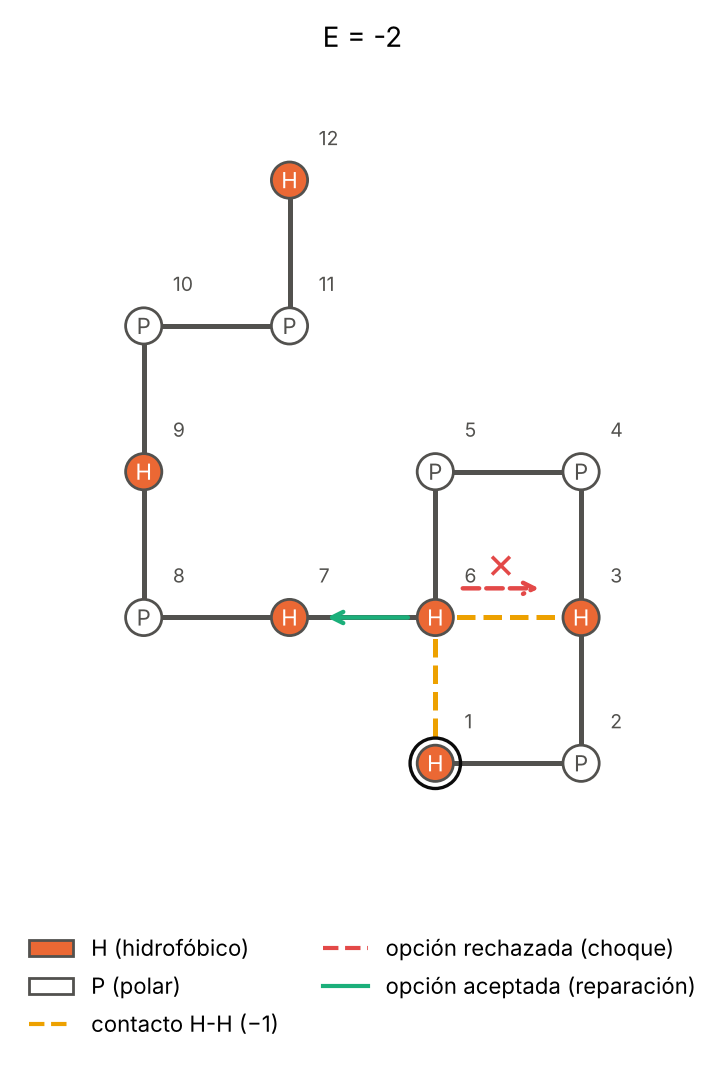
\includegraphics[width=0.55\textwidth]{figuras/hp_decodificacion_ejemplo.png}
\caption{Conformación que resulta de la Tabla~\ref{tab:decodificacion}. Los números indican la posición de cada aminoácido en la cadena. En el paso 5, girar a la izquierda desde el aminoácido 6 chocaría con el aminoácido 3 (flecha punteada), y la cadena gira a la derecha (flecha continua). La energía es $-2$, por los contactos 1--6 y 3--6.}
\label{fig:decodificacion}
\end{figure}

\subsubsection{Función de aptitud}

Si la cadena se coloca completa, la aptitud es la energía de la Ecuación~\eqref{eq:energia_hp}. Si queda encerrada después de colocar $k < n$ aminoácidos, la aptitud es
\begin{equation}
F = E_{\text{parcial}} + (n + 1)(n - k),
\label{eq:aptitud}
\end{equation}
donde $E_{\text{parcial}}$ es la energía de la parte colocada. Esta penalización garantiza que cualquier cadena incompleta sea peor que cualquier cadena completa. En la red cuadrada, los extremos tienen a lo más tres vecinos libres y los aminoácidos interiores dos, y cada contacto ocupa dos de esos lugares, así que una cadena tiene a lo más $n+1$ contactos y $E_{\text{parcial}} \ge -(n+1)$. Con $k < n$, la penalización vale al menos $n+1$ y $F \ge 0$, mientras que toda conformación completa tiene $E \le 0$. La penalización también crece con el número de aminoácidos que faltan, de modo que entre dos cadenas encerradas es mejor la que llegó más lejos. Con la reparación, estos casos son raros.

\subsubsection{Implementación y verificación}

El Código~\ref{cod:decodificar} muestra el decodificador. Las celdas ocupadas se guardan en una matriz de $(2n+3) \times (2n+3)$ centrada en el origen, suficiente aunque la cadena se estire por completo en cualquier dirección; la matriz se reutiliza entre partículas y solo se limpian las celdas que se usaron. La energía se calcula revisando, para cada aminoácido H, sus cuatro vecinos en la matriz y contando los H que estén más adelante en la cadena y no sean consecutivos.

\begin{lstlisting}[caption={Decodificación de las preferencias de una partícula.}, label={cod:decodificar}]
@njit
def decodificar(pref, es_h, DX, DY, GIRO, grid, coords):
    n = es_h.shape[0]
    off = n + 1
    coords[0, 0] = 0; coords[0, 1] = 0
    coords[1, 0] = 1; coords[1, 1] = 0
    grid[off, off] = 0
    grid[off + 1, off] = 1
    d, colocados = 0, 2
    for k in range(n - 2):
        orden = np.argsort(-pref[k])     # de mayor a menor
        ok = False
        for t in range(3):
            nd = (d + GIRO[orden[t]]) % 4
            x = coords[colocados - 1, 0] + DX[nd]
            y = coords[colocados - 1, 1] + DY[nd]
            if grid[x + off, y + off] == -1:   # celda libre
                d = nd
                coords[colocados, 0] = x; coords[colocados, 1] = y
                grid[x + off, y + off] = colocados
                colocados += 1
                ok = True
                break
        if not ok:                        # cadena encerrada
            break
    e = 0
    for i in range(colocados):
        if not es_h[i]:
            continue
        for dd in range(4):
            j = grid[coords[i, 0] + DX[dd] + off, coords[i, 1] + DY[dd] + off]
            if j > i + 1 and es_h[j]:
                e -= 1
    for i in range(colocados):            # limpiar la cuadrícula
        grid[coords[i, 0] + off, coords[i, 1] + off] = -1
    aptitud = e + (n + 1) * (n - colocados)
    return aptitud, e, colocados
\end{lstlisting}

Antes de optimizar, comprobamos que la energía estuviera bien calculada. Para la cadena \texttt{HPHPPHHPHPPH} recorrimos las $3^{10} = 59\,049$ descripciones, construimos para cada una la partícula equivalente (preferencia 1 en la opción elegida y 0 en las demás) y comparamos la energía del decodificador con la de una función independiente escrita con diccionarios de Python. No hubo ninguna diferencia en las 30\,073 conformaciones válidas, y la búsqueda exhaustiva dio el óptimo exacto de esa cadena, $E^* = -5$.

%%%%%%%%%%%%%%%%%%%%%%%%%%%%%%%%%%%%%%%%%%%%%%%%%%%%%
\subsection{Movimiento del enjambre}
\label{sec:movimiento}

Las posiciones iniciales se generan uniformes en $[0,1]^D$ y las velocidades uniformes en $[-V_{max}, V_{max}]^D$, con $V_{max} = 0.4$. Después de cada actualización, cada componente de la velocidad se limita a $[-V_{max}, V_{max}]$. Si una preferencia sale de $[0,1]$, se regresa al borde y su velocidad se invierte y se reduce a la mitad, para que la partícula no siga empujando contra la pared.

Elegimos $V_{max} = 0.4$ en pruebas preliminares con las cadenas S1-20 y S5-48, donde dio mejores resultados que 0.2. Una velocidad alta tiene sentido en esta representación porque lo que importa es el orden de las tres preferencias de cada paso: para cambiar una decisión, una preferencia tiene que rebasar a otra, y con velocidades pequeñas eso tarda muchas iteraciones.

Las mejores posiciones personales se actualizan cuando la nueva aptitud es menor \textit{o igual} que la anterior. Con la comparación estricta, una partícula que encuentra otra conformación con la misma energía no la recuerda. Con la comparación no estricta, el \textit{pbest} puede moverse a lo largo de una meseta del paisaje (Sección~\ref{sec:dificultad}), y eso le da al enjambre una forma de seguir explorando cuando la energía no cambia.

%%%%%%%%%%%%%%%%%%%%%%%%%%%%%%%%%%%%%%%%%%%%%%%%%%%%%
\subsection{Estrategia de los coeficientes}
\label{sec:estrategia}

\subsubsection{Curva coseno}

Los tres coeficientes se mueven entre los valores de la Tabla~\ref{tab:coeficientes} con la curva coseno de la Ecuación~\eqref{eq:coseno}:
\begin{align}
w(s)   &= w_f + (w_i - w_f)\, g(s), \label{eq:w_cos}\\
c_1(s) &= c_{1f} + (c_{1i} - c_{1f})\, g(s), \label{eq:c1_cos}\\
c_2(s) &= c_{2f} + (c_{2i} - c_{2f})\, g(s), \label{eq:c2_cos}
\end{align}
donde $s \in [0,1]$ es la fase de la búsqueda. Los extremos son los del esquema TVAC~\cite{shi1999empirical, ratnaweera2004self}, y con ellos $c_1 + c_2 = 3$ en todo momento: lo que pierde la atracción hacia la memoria propia lo gana la atracción hacia el enjambre.

\begin{table}[H]
\centering
\caption{Valores inicial y final de los coeficientes.}
\label{tab:coeficientes}
\begin{tabular}{lcc}
\toprule
Coeficiente & Inicio ($s = 0$) & Final ($s = 1$) \\
\midrule
$w$   & 0.9 & 0.4 \\
$c_1$ & 2.5 & 0.5 \\
$c_2$ & 0.5 & 2.5 \\
\bottomrule
\end{tabular}
\end{table}

Elegimos la curva coseno por la forma del paisaje del modelo HP. Como está lleno de mesetas, el enjambre necesita mucho tiempo explorando antes de concentrarse. Una curva exponencial reduce $w$ muy rápido al inicio y deja poco tiempo de exploración. Una curva lineal reparte el tiempo por igual. La curva coseno cambia despacio al inicio, así que mantiene $w$ y $c_1$ altos durante una fase larga de exploración; hace la transición rápida a la mitad, y vuelve a cambiar despacio al final, con una fase larga de refinamiento con $c_2$ alto. La Figura~\ref{fig:curvas} compara las tres curvas.

\begin{figure}[H]
\centering
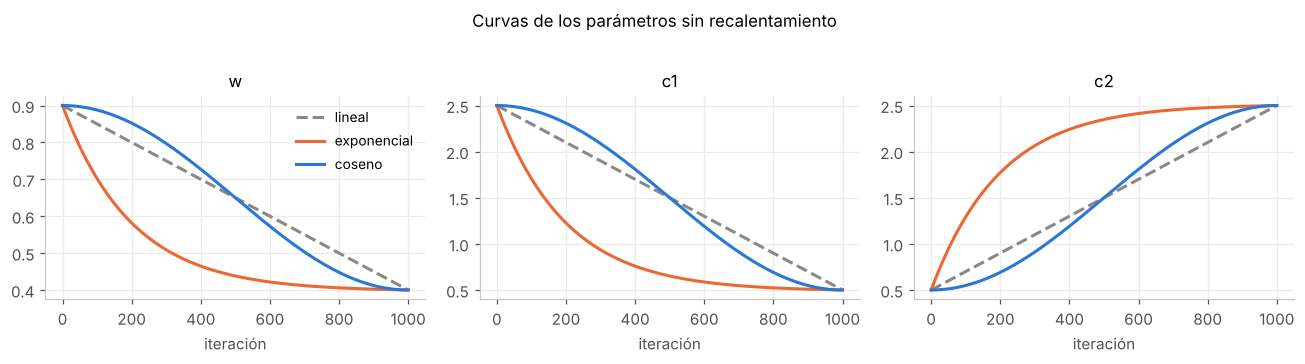
\includegraphics[width=\textwidth]{figuras/hp_curvas_parametros.png}
\caption{Valores de $w$, $c_1$ y $c_2$ a lo largo de 1000 iteraciones con las curvas lineal, exponencial y coseno, sin recalentamiento.}
\label{fig:curvas}
\end{figure}

Según la condición de Poli (Ecuación~\eqref{eq:poli}), con $w = 0.4$ el límite para $c_1 + c_2$ es $24(1 - 0.16)/(7 - 2) = 4.03$, mayor que 3, así que al final de la búsqueda las partículas convergen. Con $w = 0.9$ el límite es $24(1 - 0.81)/(7 - 4.5) = 1.82$, menor que 3, y al inicio las partículas no se estabilizan. Esto es intencional: al principio buscamos exploración amplia, y la velocidad máxima evita que las oscilaciones crezcan sin control.

\subsubsection{Recalentamiento por estancamiento}

Una curva fija no sabe si el enjambre está mejorando o no. Para que los coeficientes reaccionen al estado de la búsqueda, la fase se calcula como
\begin{equation}
s(t) = \frac{t}{T} - b(t),
\label{eq:fase}
\end{equation}
donde $t$ es la iteración, $T$ el total de iteraciones y $b(t) \ge 0$ un retroceso que empieza en cero. En cada iteración $b$ se multiplica por un factor de decaimiento $\delta = 0.98$. Si \textit{gbest} pasa $p = 50$ iteraciones sin mejorar, se suma un impulso $\beta = 0.5$:
\begin{equation}
b \leftarrow \min\!\left(b + \beta,\ \tfrac{t}{T}\right),
\label{eq:recalentar}
\end{equation}
y el contador de iteraciones sin mejora vuelve a cero. El límite $t/T$ evita que la fase sea negativa. Al recalentar, la fase retrocede, $w$ y $c_1$ vuelven a subir y $c_2$ baja, así que el enjambre recupera capacidad de exploración sin perder sus memorias. Como $b$ decae alrededor de 2\,\% por iteración, el efecto se reduce a la mitad en unas 34 iteraciones y los coeficientes regresan solos a la tendencia de la curva.

La primera versión de este mecanismo era distinta: en cada estancamiento multiplicaba la fase por 0.5, sin ningún decaimiento. Al graficar los coeficientes usados en las 30 ejecuciones vimos que los estancamientos ocurrían tan seguido que la fase nunca pasaba de alrededor de 0.1, y $w$ se quedaba cerca de 0.88 durante toda la ejecución. En la práctica, la curva coseno no se estaba aplicando. Con la versión de la Ecuación~\eqref{eq:fase} el retroceso es temporal y la curva conserva su forma. En las 30 ejecuciones los resultados de las dos versiones fueron muy parecidos: la media final de la versión corregida fue mejor en S4-36 ($-12.33$ contra $-12.30$), S5-48 ($-18.73$ contra $-18.43$) y S8-64 ($-29.73$ contra $-28.90$), y un poco peor en S1-20 ($-8.67$ contra $-8.73$). Aun así, el hecho de que la primera versión funcionara bien con $w$ casi constante y alto nos dio una pista sobre el problema: en el modelo HP conviene explorar durante mucho tiempo.

%%%%%%%%%%%%%%%%%%%%%%%%%%%%%%%%%%%%%%%%%%%%%%%%%%%%%
\subsection{Medidas de diversidad}
\label{sec:diversidad_impl}

En cada iteración calculamos las tres medidas de la Ecuación~\eqref{eq:diversidad}. Como las cadenas tienen distinto número de dimensiones, las normalizamos para poder compararlas: la diversidad de posición y la cognitiva se dividen entre $\sqrt{D}$, que es la diagonal del hipercubo $[0,1]^D$, y la de velocidad entre $V_{max}\sqrt{D}$. Con esta normalización, un enjambre con posiciones uniformes al azar tiene diversidad de posición cercana a $\sqrt{1/12} \approx 0.29$ (la desviación estándar de una variable uniforme en $[0,1]$), y velocidades uniformes en $[-V_{max}, V_{max}]$ dan una diversidad de velocidad cercana a $\sqrt{1/3} \approx 0.58$. Esos son los valores de la iteración 0 y sirven como referencia para interpretar las gráficas.

%%%%%%%%%%%%%%%%%%%%%%%%%%%%%%%%%%%%%%%%%%%%%%%%%%%%%
\subsection{Algoritmo completo}

El Código~\ref{cod:pso} muestra el ciclo principal de una ejecución.

\begin{lstlisting}[caption={Ciclo principal de PSO (fragmento).}, label={cod:pso}]
for t in range(1, T + 1):
    w, c1, c2 = parametros(s, cfg)
    r1, r2 = rng.random((P, D)), rng.random((P, D))
    V = w * V + c1 * r1 * (pbest - X) + c2 * r2 * (gbest - X)
    np.clip(V, -vmax, vmax, out=V)
    X = X + V
    fuera = (X < 0) | (X > 1)
    V[fuera] *= -0.5
    np.clip(X, 0.0, 1.0, out=X)

    f = evaluar_enjambre(X, es_h, DX, DY, GIRO)
    mejora = f <= pfit                      # acepta empates
    pbest[mejora], pfit[mejora] = X[mejora], f[mejora]
    g = int(np.argmin(pfit))
    if pfit[g] < gfit:
        gbest, gfit = pbest[g].copy(), pfit[g]
        sin_mejora = 0
    else:
        sin_mejora += 1

    b *= cfg["decaimiento"]                 # recalentamiento
    if sin_mejora >= cfg["paciencia"]:
        b = min(b + cfg["impulso"], t / T)
        sin_mejora = 0
    s = t / T - b
    registrar(t)                            # gbest y las tres diversidades
\end{lstlisting}

%%%%%%%%%%%%%%%%%%%%%%%%%%%%%%%%%%%%%%%%%%%%%%%%%%%%%
\subsection{Ejemplo: evolución de una partícula}
\label{sec:ejemplo_particula}

Para ilustrar cómo mejora una partícula, la Figura~\ref{fig:evolucion} muestra cuatro momentos hipotéticos de su recorrido sobre la cadena \texttt{HPHPPHHPHPPH}, cuyo óptimo es $-5$. Los números de iteración son ilustrativos, pero las conformaciones y sus energías son reales: las calculamos con el decodificador. Debajo de cada conformación está la decisión ganadora de cada paso.

\begin{figure}[H]
\centering
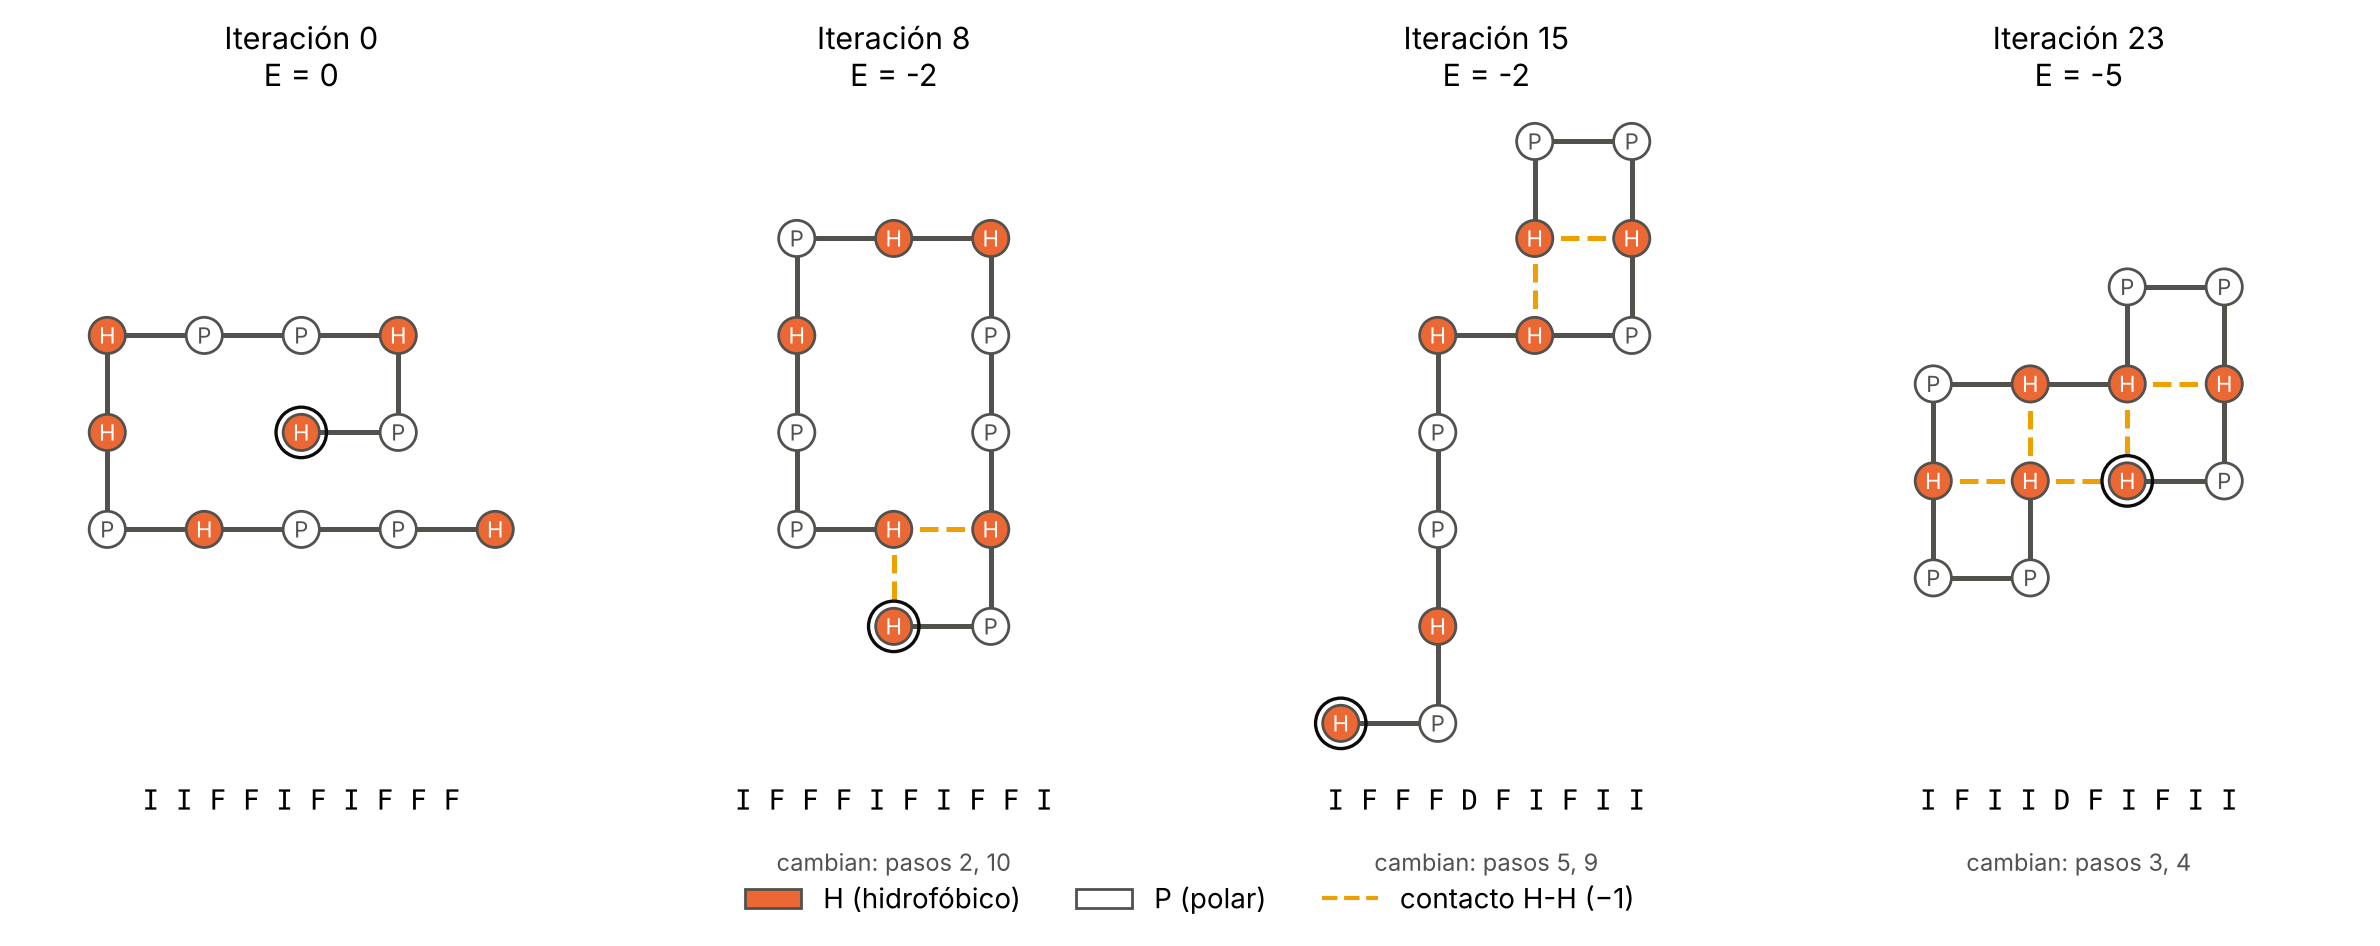
\includegraphics[width=\textwidth]{figuras/hp_evolucion_particula.png}
\caption{Cuatro momentos de una partícula sobre la cadena HPHPPHHPHPPH. Debajo de cada conformación están las decisiones de los diez pasos (I = izquierda, F = frente, D = derecha) y los pasos que cambiaron respecto al momento anterior.}
\label{fig:evolucion}
\end{figure}

En la iteración 0 las preferencias son aleatorias. La cadena queda casi estirada, en forma de gancho, y ninguna H toca a otra H que no sea su vecina en la cadena, así que la energía es 0. Esta forma se guarda como su \textit{pbest}, porque es la única que conoce.

Para la iteración 8 las preferencias se movieron hacia el \textit{gbest} del enjambre. Cambiaron solo dos decisiones, los pasos 2 y 10, y eso bastó para doblar la cadena en forma de U: la última H queda junto a la primera y a la tercera. La energía baja a $-2$ y esta forma se convierte en el nuevo \textit{pbest}.

En la iteración 15 la partícula prueba una forma bastante distinta, después de cambiar los pasos 5 y 9. Ahora los contactos están en otra parte de la cadena, pero la energía sigue en $-2$. No todos los movimientos mejoran, y que la partícula pruebe formas distintas con la misma energía es parte de cómo el enjambre explora las mesetas. Como aceptamos empates en el \textit{pbest}, esta forma también puede guardarse.

En la iteración 23, al cambiar los pasos 3 y 4, la cadena se cierra sobre sí misma y las H quedan agrupadas en el centro, con cinco contactos. Es la energía mínima de esta cadena. Entre momentos sucesivos solo cambian dos de las diez decisiones, porque las preferencias se mueven de forma gradual y una decisión cambia solo cuando una preferencia rebasa a otra.

%%%%%%%%%%%%%%%%%%%%%%%%%%%%%%%%%%%%%%%%%%%%%%%%%%%%%
\subsection{Diseño experimental}
\label{sec:diseno}

Usamos 80 partículas y 1000 iteraciones en todas las cadenas. Elegimos estos valores en pruebas preliminares de 8 ejecuciones: con 50 partículas y $V_{max} = 0.2$ el algoritmo no encontró el óptimo de S1-20 en ninguna, y con 80 partículas y $V_{max} = 0.4$ lo encontró en la mitad de ellas y mejoró la media en S5-48. El tiempo de cómputo no fue un problema: las 30 ejecuciones tardaron entre 21 y 61 segundos por cadena.

Cada cadena se ejecutó 30 veces, con las semillas $2026 + r$ para $r = 0, \dots, 29$. En cada iteración guardamos \textit{gbest}, las tres medidas de diversidad y los valores de $w$, $c_1$ y $c_2$ realmente usados. Con las 30 ejecuciones calculamos la media y la desviación estándar muestral de cada cantidad en cada iteración. También registramos, para cada ejecución, la iteración en la que alcanzó su valor final de \textit{gbest} y el número de recalentamientos.

Para justificar la estrategia de coeficientes, comparamos cuatro variantes con la misma configuración y las mismas semillas: curva lineal, curva exponencial ($g(s) = (e^{-5s} - e^{-5})/(1 - e^{-5})$), curva coseno sin recalentamiento y curva coseno con recalentamiento. Esta comparación la hicimos en las cadenas S1-20 y S4-36, con 30 ejecuciones por variante. Para cada variante aplicamos la prueba de Mann-Whitney unilateral contra la estrategia elegida, con la hipótesis alternativa de que la estrategia elegida obtiene energías finales menores, usando la función \texttt{mannwhitneyu} de SciPy y $\alpha = 0.05$.
